\documentclass[11pt,a4paper]{article}
\input{estilo-relatorio}

\roteiro{1}{Simulação de Circuitos: Introdução ao LTspice}
\aturma{04}
\autorum{Gabriel de Sousa}{211056000}

\usepackage{placeins}
\renewcommand{\topfraction}{0.92}
\renewcommand{\bottomfraction}{0.85}
\renewcommand{\textfraction}{0.08}
\renewcommand{\floatpagefraction}{0.75}
\setcounter{topnumber}{3}
\setcounter{bottomnumber}{2}
\setcounter{totalnumber}{5}

\begin{document}
\capa

\begin{resumo}
Este relatório apresenta o projeto e a análise de quatro topologias elementares a partir dos
arquivos associados à matrícula 211056000: divisor resistivo com carga, filtro RC passa-baixas,
circuito RLC série e filtro RC excitado por onda quadrada. No divisor, a saída calculada passa de
\SI{6,471}{\volt} sem carga para \SI{3,642}{\volt} com \SI{1}{\kilo\ohm}. O filtro RC possui
frequência de corte efetiva de \SI{408,1}{\hertz}, \SI{5,18}{\percent} acima da referência de
\SI{388}{\hertz}. No RLC, resistências de \SI{4,7}{\kilo\ohm}, \SI{12}{\kilo\ohm} e
\SI{22}{\kilo\ohm} produzem fatores de amortecimento de 0,235, 0,600 e 1,100. A análise da onda
quadrada evidencia a atenuação crescente das harmônicas ímpares. Os resultados confirmam as
expressões analíticas para componentes ideais e mostram a influência da carga, da série E12 e do
amortecimento.
\end{resumo}

\section{Introdução}

Divisores de tensão, filtros passivos e circuitos ressonantes são usados no condicionamento de
sinais, na polarização de dispositivos e na seleção de faixas de frequência. Mesmo com poucos
componentes, essas redes podem se afastar do comportamento desejado quando a carga não é
considerada, quando os componentes comerciais diferem do valor ideal ou quando a dissipação não é
suficiente para amortecer a energia armazenada.

O LTspice permite verificar essas condições antes da montagem. Neste roteiro são usadas análises de
ponto de operação, varredura DC, resposta em frequência, resposta ao degrau e conteúdo espectral.
Os esquemáticos e os gráficos deste documento são capturas de tela do próprio LTspice, obtidas
dos arquivos \texttt{item\_1.asc} a \texttt{item\_6.asc}.

O objetivo é dimensionar e caracterizar as topologias definidas nos arquivos do autor, comparando as
previsões analíticas com as respostas de projeto. A Seção 2 apresenta as relações teóricas, a Seção 3
detalha os componentes escolhidos, a Seção 4 descreve as simulações, e as Seções 5 a 7 apresentam,
discutem e sintetizam os resultados.

\section{Fundamentação teórica}

\subsection{Divisor resistivo com carga}

O circuito formado por $V_{in}$, $R_1$ e $R_2$ pode ser substituído, do ponto de vista da carga, por
seu equivalente de Thévenin:
\begin{equation}
V_{th}=V_{in}\frac{R_2}{R_1+R_2}, \qquad
R_{th}=R_1\parallel R_2=\frac{R_1R_2}{R_1+R_2}.
\label{eq:thevenin}
\end{equation}
Com $R_L$ conectado, a saída e sua queda relativa são
\begin{equation}
V_{carga}=V_{th}\frac{R_L}{R_L+R_{th}}, \qquad
\delta_V=\frac{V_{th}-V_{carga}}{V_{th}}=\frac{R_{th}}{R_L+R_{th}}.
\label{eq:carga}
\end{equation}

\subsection{Filtro RC passa-baixas}

Tomando a saída sobre o capacitor, a função de transferência do filtro é
\begin{equation}
H(j\omega)=\frac{V_{out}}{V_{in}}=\frac{1}{1+j\omega RC}, \qquad
f_c=\frac{1}{2\pi RC}.
\label{eq:rc}
\end{equation}
O ganho e a fase são
\begin{equation}
G_{dB}=-10\log_{10}\left[1+\left(\frac{f}{f_c}\right)^2\right], \qquad
\phi=-\arctan\left(\frac{f}{f_c}\right).
\label{eq:bode-rc}
\end{equation}
Em $f_c$, o ganho é \SI{-3,01}{\decibel} e a fase é $-45^\circ$. Em alta frequência, a
inclinação tende a \SI{-20}{\decibel} por década.

\subsection{Circuito RLC série}

Para a saída sobre o capacitor,
\begin{equation}
H(s)=\frac{1}{LCs^2+RCs+1}.
\end{equation}
A frequência natural, o fator de amortecimento e a resistência crítica são
\begin{equation}
f_0=\frac{1}{2\pi\sqrt{LC}}, \qquad
\zeta=\frac{R}{2}\sqrt{\frac{C}{L}}, \qquad
R_{crit}=2\sqrt{\frac{L}{C}}.
\label{eq:rlc}
\end{equation}
Para $\zeta<1$, a frequência amortecida e o sobressinal do degrau são
\begin{equation}
f_d=f_0\sqrt{1-\zeta^2}, \qquad
M_p=\exp\left(\frac{-\pi\zeta}{\sqrt{1-\zeta^2}}\right)100\%.
\label{eq:degrau}
\end{equation}
O pico de ressonância existe quando $\zeta<1/\sqrt{2}$ e ocorre em
\begin{equation}
f_r=f_0\sqrt{1-2\zeta^2}, \qquad
|H|_{max}=\frac{1}{2\zeta\sqrt{1-\zeta^2}}.
\label{eq:ressonancia}
\end{equation}

\subsection{Onda quadrada}

Uma onda quadrada bipolar de amplitude $A$ possui somente harmônicas ímpares, com amplitude
\begin{equation}
V_n=\frac{4A}{n\pi}, \qquad n=1,3,5,\ldots
\label{eq:fourier}
\end{equation}
Após o filtro, cada componente é multiplicada por $|H(j2\pi nf_1)|$. Por isso as harmônicas mais
altas são removidas mais intensamente e as bordas do sinal ficam arredondadas.

\section{Especificação e projeto}

\begin{espec}
Matrícula \mat{211056000}. Valores registrados nos arquivos do autor: tensão carregada de
referência $2+56/33=\SI{3,697}{\volt}$; queda mínima de 25\%; frequência de referência do filtro
$f_c=\SI{388}{\hertz}$; $L=\SI{100}{\milli\henry}$; $C_{RLC}=\SI{1}{\nano\farad}$; resistência
central do RLC de \SI{12}{\kilo\ohm}; onda quadrada com $f_1\approx\SI{388}{\hertz}$.
\end{espec}

No divisor foram usados $R_1=\SI{1,2}{\kilo\ohm}$, $R_2=\SI{2,2}{\kilo\ohm}$ e
$R_L=\SI{1}{\kilo\ohm}$. As Equações~\ref{eq:thevenin} e \ref{eq:carga} fornecem
$R_{th}=\SI{776,47}{\ohm}$, $V_{th}=\SI{6,4706}{\volt}$ e
$V_{carga}=\SI{3,6424}{\volt}$. A saída carregada fica 1,48\% abaixo da referência e a queda
relativa é 43,71\%, atendendo ao mínimo pedido.

No filtro, $C=\SI{100}{\nano\farad}$ exigiria $R_{ideal}=\SI{4,101}{\kilo\ohm}$ para
\SI{388}{\hertz}. O valor E12 adotado foi \SI{3,9}{\kilo\ohm}, que produz
$f_{c,efetiva}=\SI{408,09}{\hertz}$, desvio de +5,18\%.

No RLC, $L=\SI{100}{\milli\henry}$ e $C=\SI{1}{\nano\farad}$ fixam
$f_0=\SI{15,915}{\kilo\hertz}$ e $R_{crit}=\SI{20}{\kilo\ohm}$. A varredura de $R$ foi escolhida
para mostrar respostas subamortecidas e superamortecidas.

\begin{center}
\begin{tabular}{@{}lrrr@{}}
\toprule
\textbf{Grandeza} & \textbf{Teórico} & \textbf{Adotado} & \textbf{Desvio} \\
\midrule
$V_{carga}$ & \SI{3,697}{\volt} & \SI{3,642}{\volt} & $-1,48$\% \\
$R$ do RC & \SI{4,101}{\kilo\ohm} & \SI{3,9}{\kilo\ohm} & $-4,90$\% \\
$f_c$ do RC & \SI{388}{\hertz} & \SI{408,09}{\hertz} & $+5,18$\% \\
$R$ central do RLC & \SI{12}{\kilo\ohm} & \SI{12}{\kilo\ohm} & 0\% \\
\bottomrule
\end{tabular}
\end{center}

\section{Metodologia}

\subsection{Simulação de projeto, uma por integrante}

Os itens 1 e 2 usam o divisor das Figuras~\ref{fig:divisor-op} e \ref{fig:divisor}. A diretiva
\texttt{.step param RL list 1000 1000meg} representa a condição carregada e a aproximação de
circuito aberto. O item 1 executa \texttt{.op}; o item 2 varre a fonte de 0 a \SI{15}{\volt} em
passos de \SI{0,1}{\volt}.

\begin{figure}[htb]
\centering
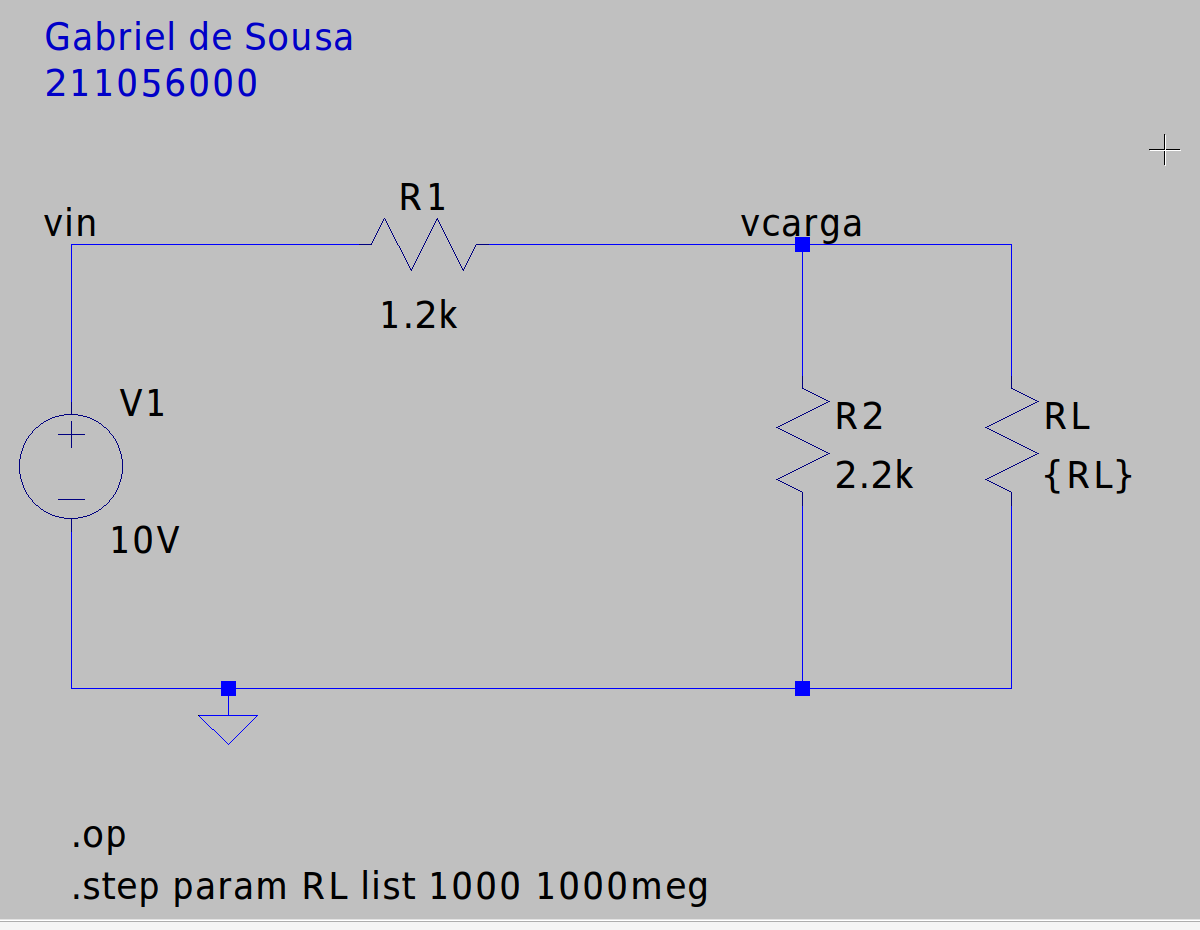
\includegraphics[width=.62\linewidth]{figuras/item_1_ltspice_op_esquematico_corte.png}
\caption{Esquemático do divisor resistivo no LTspice com a diretiva \texttt{.op}
(\texttt{item\_1.asc}), com a carga parametrizada.}
\label{fig:divisor-op}
\end{figure}

\begin{figure}[htb]
\centering
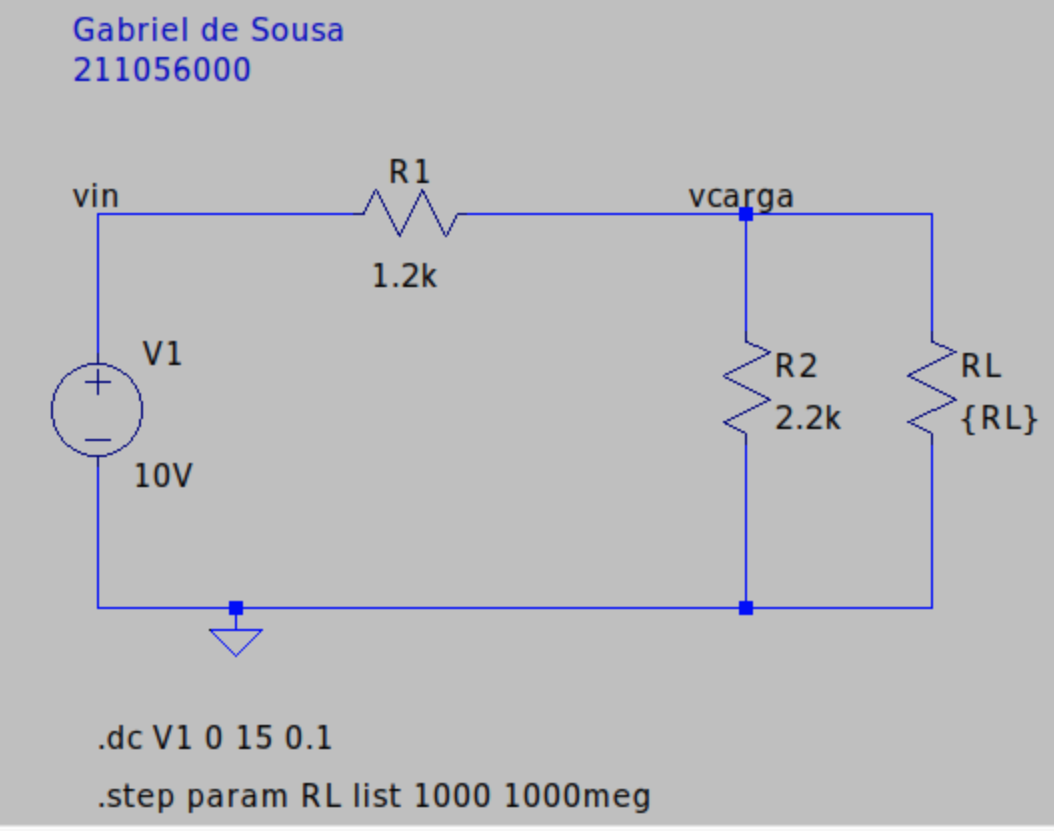
\includegraphics[width=.85\linewidth]{figuras/2.png}
\caption{Mesmo divisor com a diretiva \texttt{.dc} ativa (\texttt{item\_2.asc}).}
\label{fig:divisor}
\end{figure}

O item 3 usa o filtro da Figura~\ref{fig:rc-ac}, fonte AC de \SI{1}{\volt} e varredura
\texttt{.ac dec 100 3.88 38800}. Essa faixa cobre quatro décadas em torno da frequência de
referência.

\begin{figure}[htb]
\centering
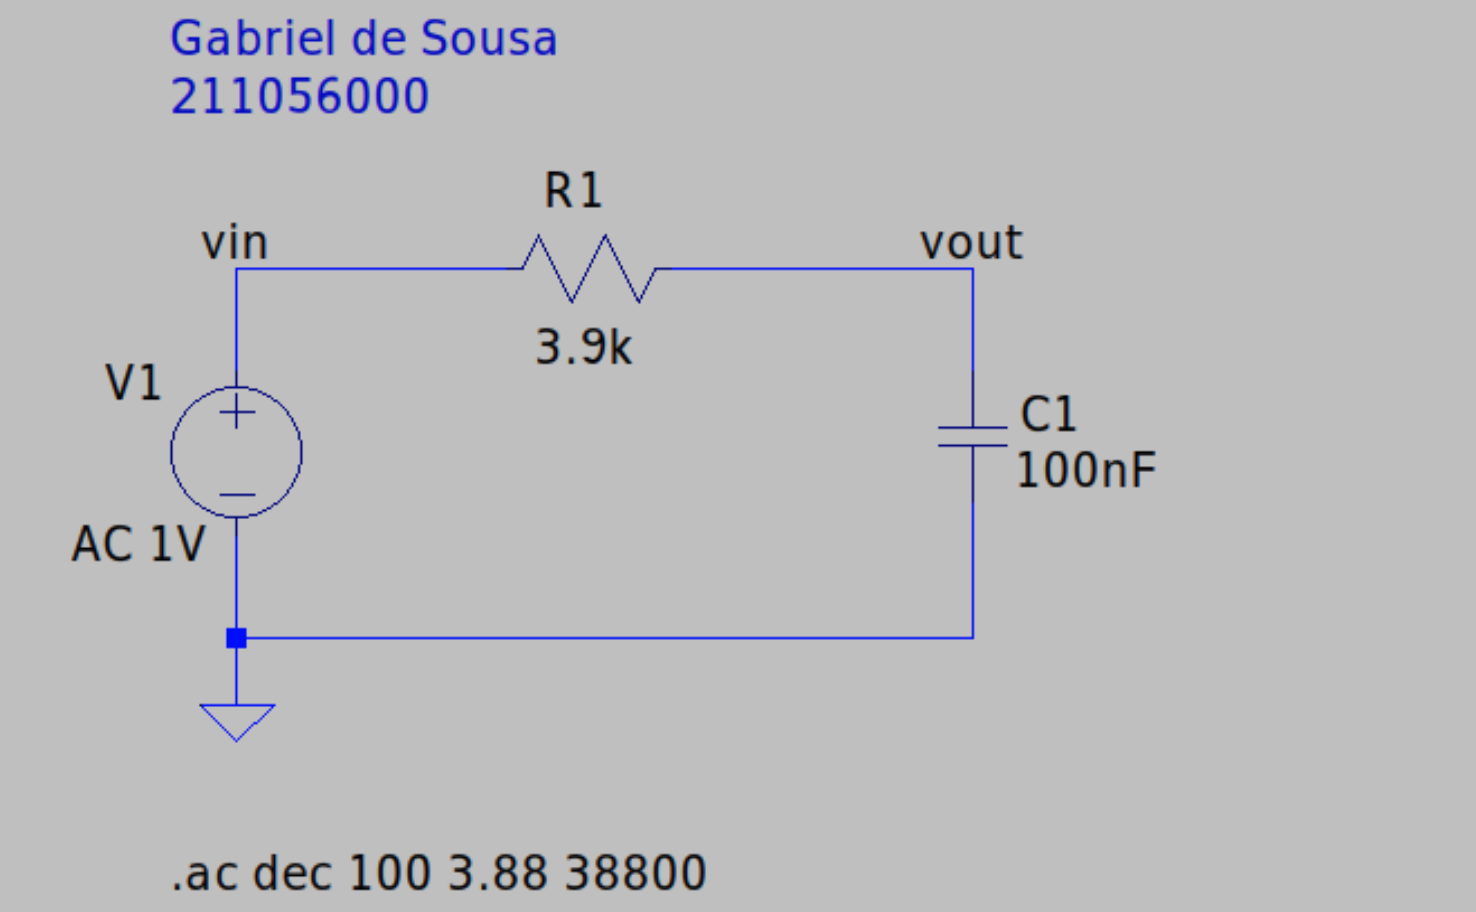
\includegraphics[width=.85\linewidth]{figuras/3.png}
\caption{Esquemático do filtro RC passa-baixas no LTspice (\texttt{item\_3.asc}).}
\label{fig:rc-ac}
\end{figure}

Nos itens 4 e 5, o RLC das Figuras~\ref{fig:rlc-esq-tran} e \ref{fig:rlc-esq-ac} usa
\texttt{.step param R list 4700 12000 22000}. O item 4 recebe um degrau e executa
\texttt{.tran 300u}; o item 5 usa amplitude AC de \SI{1}{\volt} e
\texttt{.ac dec 100 159.16 1591550}.

\begin{figure}[htb]
\centering
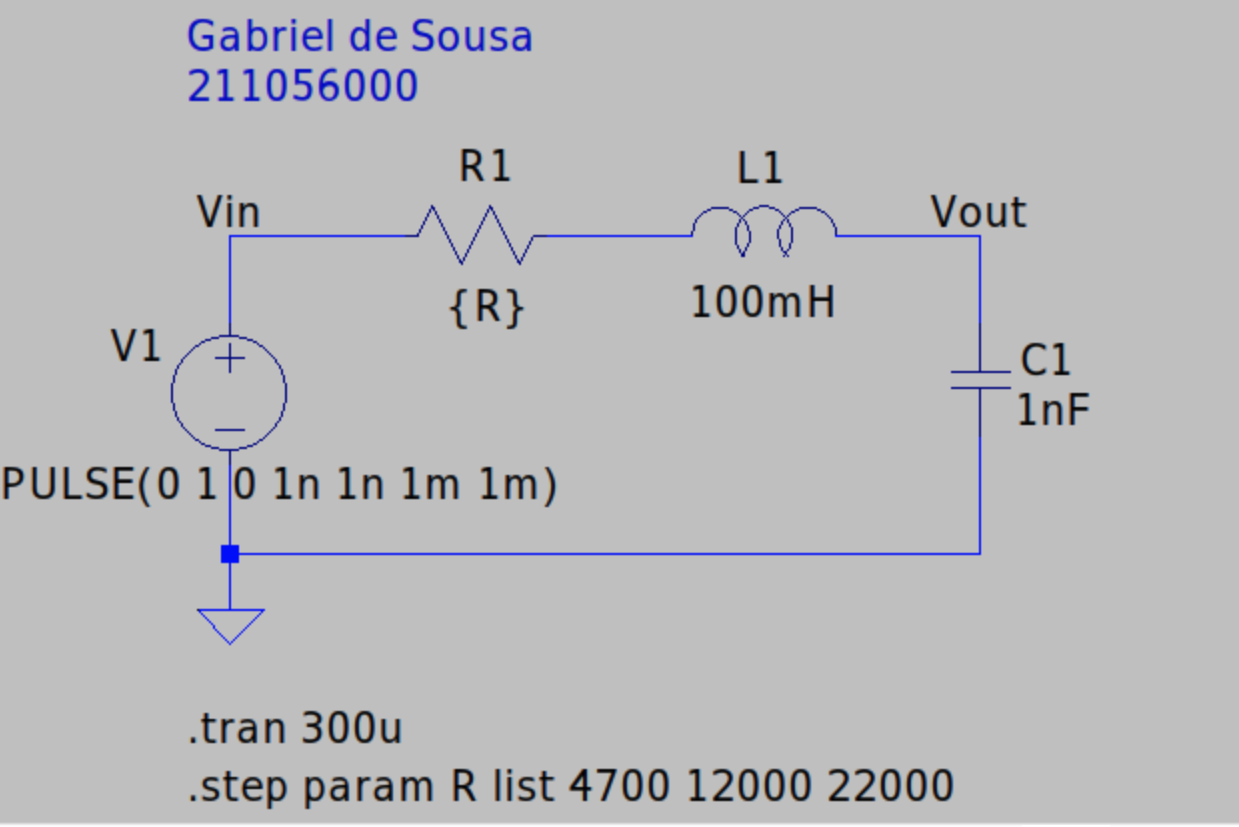
\includegraphics[width=.85\linewidth]{figuras/4.png}
\caption{Esquemático do RLC série no LTspice para a análise transiente (\texttt{item\_4.asc}).}
\label{fig:rlc-esq-tran}
\end{figure}

\begin{figure}[htb]
\centering
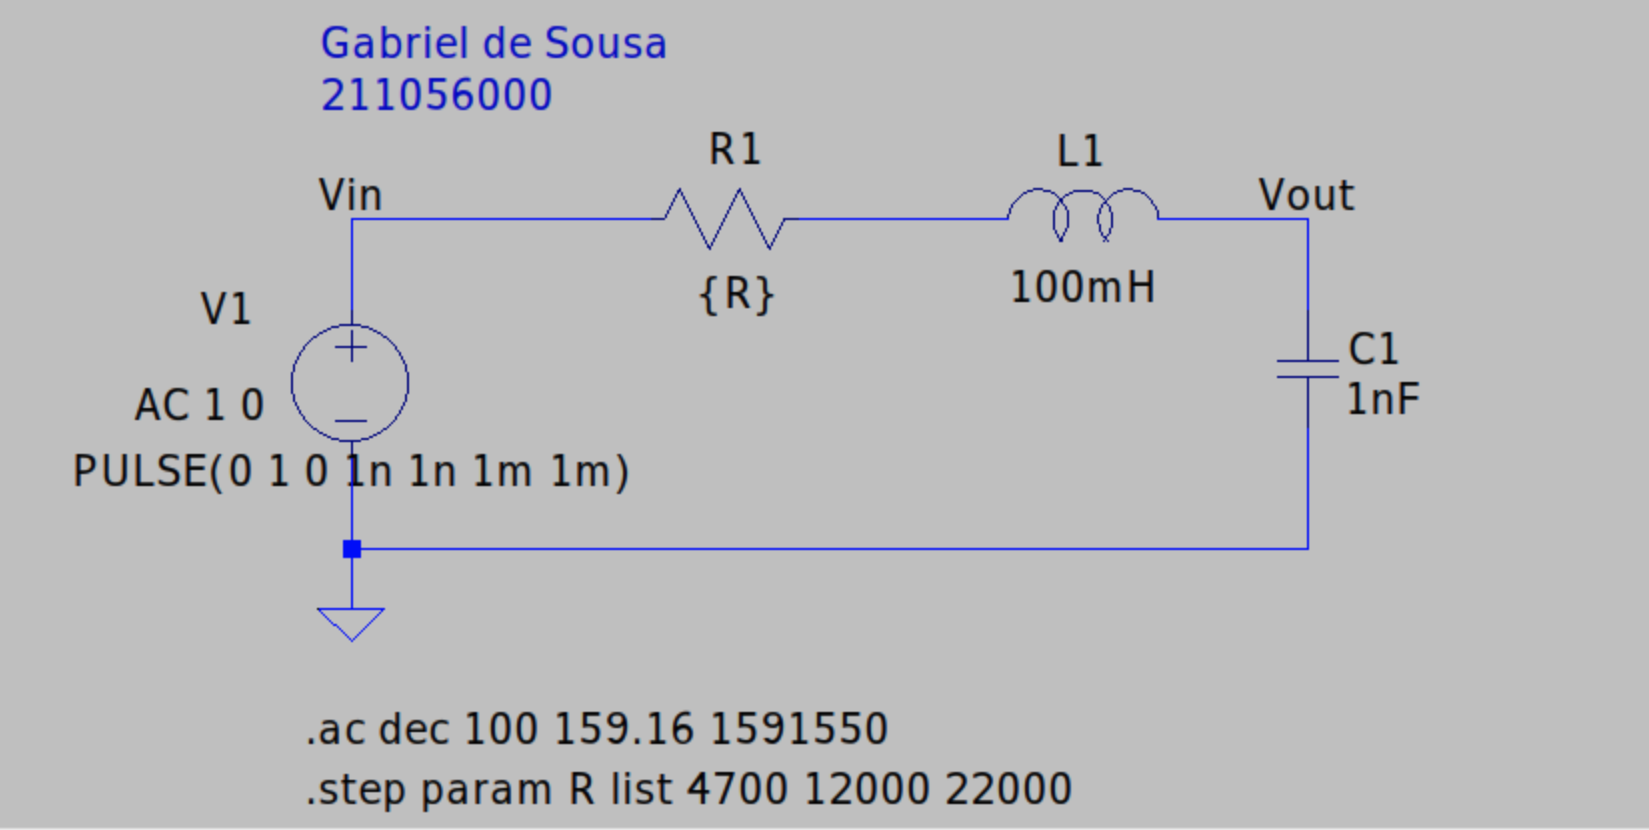
\includegraphics[width=.85\linewidth]{figuras/5.png}
\caption{Esquemático do RLC série no LTspice para a resposta em frequência (\texttt{item\_5.asc}).}
\label{fig:rlc-esq-ac}
\end{figure}

O item 6 reutiliza o RC, mas com
\texttt{PULSE(-1 1 0 1n 1n 1.2887m 2.5773m)}. A análise cobre 20 períodos, descarta os cinco
primeiros, limita o passo a \SI{8,591}{\micro\second} e desliga a compressão dos pontos.

\begin{figure}[htb]
\centering
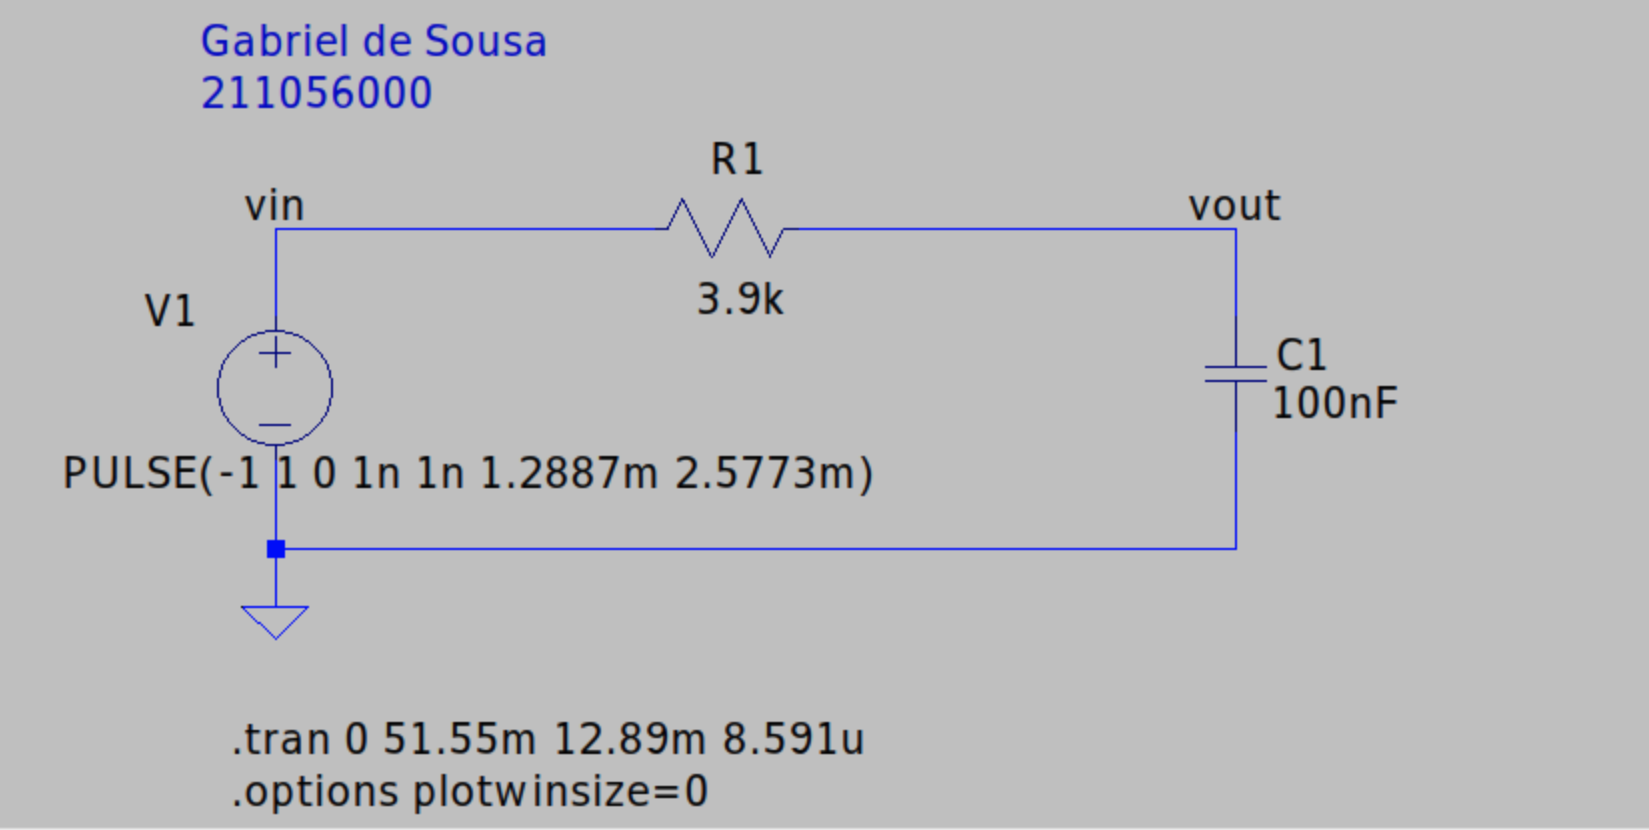
\includegraphics[width=.85\linewidth]{figuras/6.png}
\caption{Esquemático do filtro RC excitado por onda quadrada no LTspice (\texttt{item\_6.asc}).}
\label{fig:rc-pulse}
\end{figure}

\section{Resultados}

\subsection{Projeto de cada integrante}

No ponto de operação, o divisor fornece os valores da Tabela~\ref{tab:op}, lidos das janelas da Figura~\ref{fig:op}. A varredura da
Figura~\ref{fig:dc} confirma que ambas as saídas são lineares e que a razão entre elas permanece
constante.

\begin{center}
\captionof{table}{Ponto de operação do divisor para $V_1=\SI{10}{\volt}$.}
\label{tab:op}
\begin{tabular}{@{}lrr@{}}
\toprule
\textbf{Grandeza} & \textbf{$R_L=1$ k$\Omega$} & \textbf{Sem carga} \\
\midrule
$V(v_{carga})$ & \SI{3,64238}{\volt} & \SI{6,47058}{\volt} \\
Corrente da fonte & \SI{5,298}{\milli\ampere} & \SI{2,941}{\milli\ampere} \\
\bottomrule
\end{tabular}
\end{center}

\begin{figure}[htb]
\centering
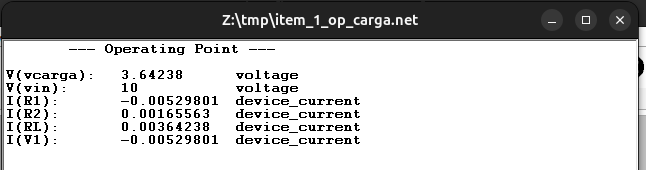
\includegraphics[width=.49\linewidth]{figuras/item_1_ltspice_op_resultado_carga_corte.png}\hfill
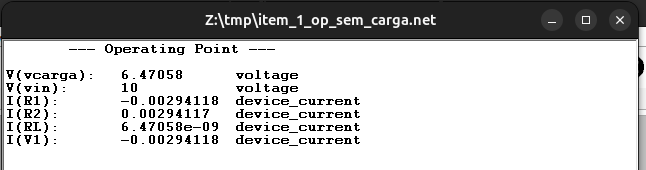
\includegraphics[width=.49\linewidth]{figuras/item_1_ltspice_op_resultado_sem_carga_corte.png}
\caption{Janelas de ponto de operação do LTspice (\texttt{item\_1.asc}): à esquerda com
$R_L=\SI{1}{\kilo\ohm}$, à direita em circuito aberto.}
\label{fig:op}
\end{figure}

\begin{figure}[htb]
\centering
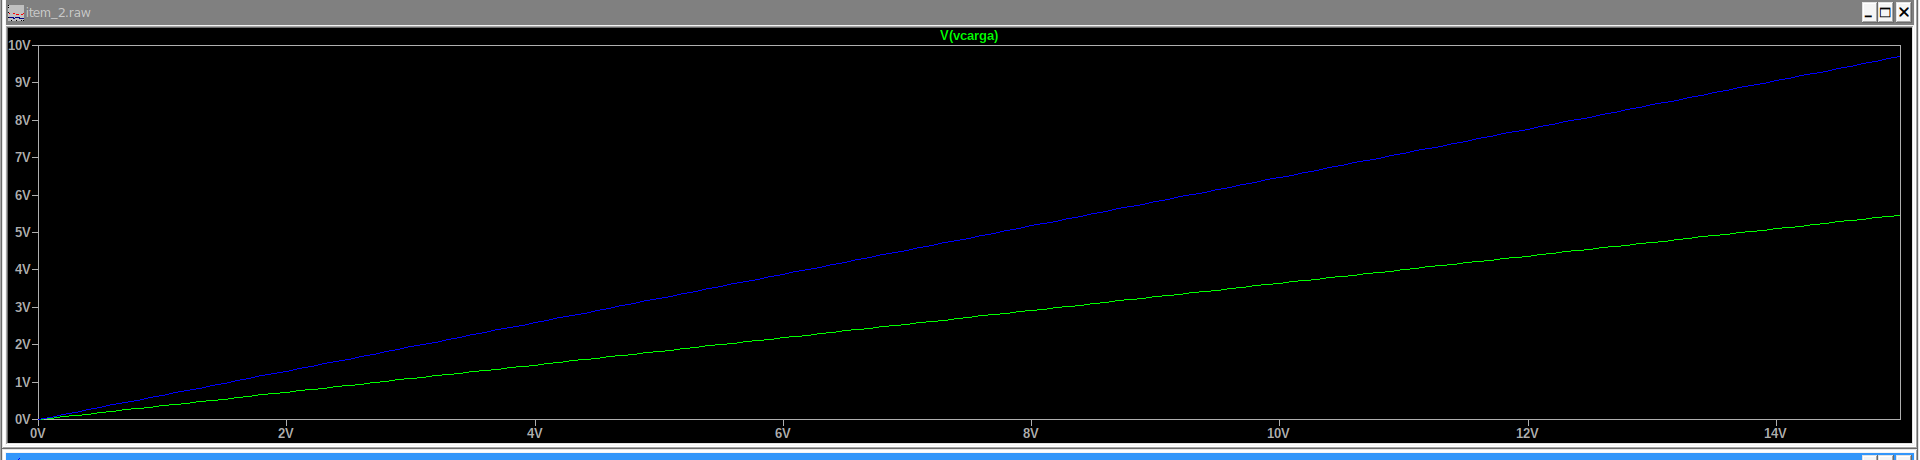
\includegraphics[width=\linewidth]{figuras/item_2_ltspice_corte.png}
\caption{Varredura DC do divisor no LTspice (\texttt{item\_2.asc}): $V(v_{carga})$ com $R_L=\SI{1}{\kilo\ohm}$ e em circuito aberto.}
\label{fig:dc}
\end{figure}

O Bode do item 3 é mostrado na Figura~\ref{fig:bode-rc}. Em
\SI{408,09}{\hertz}, o ganho é \SI{-3,010}{\decibel} e a fase é $-45^\circ$; em dez vezes essa
frequência, o ganho chega a \SI{-20,043}{\decibel}.

\begin{figure}[htb]
\centering
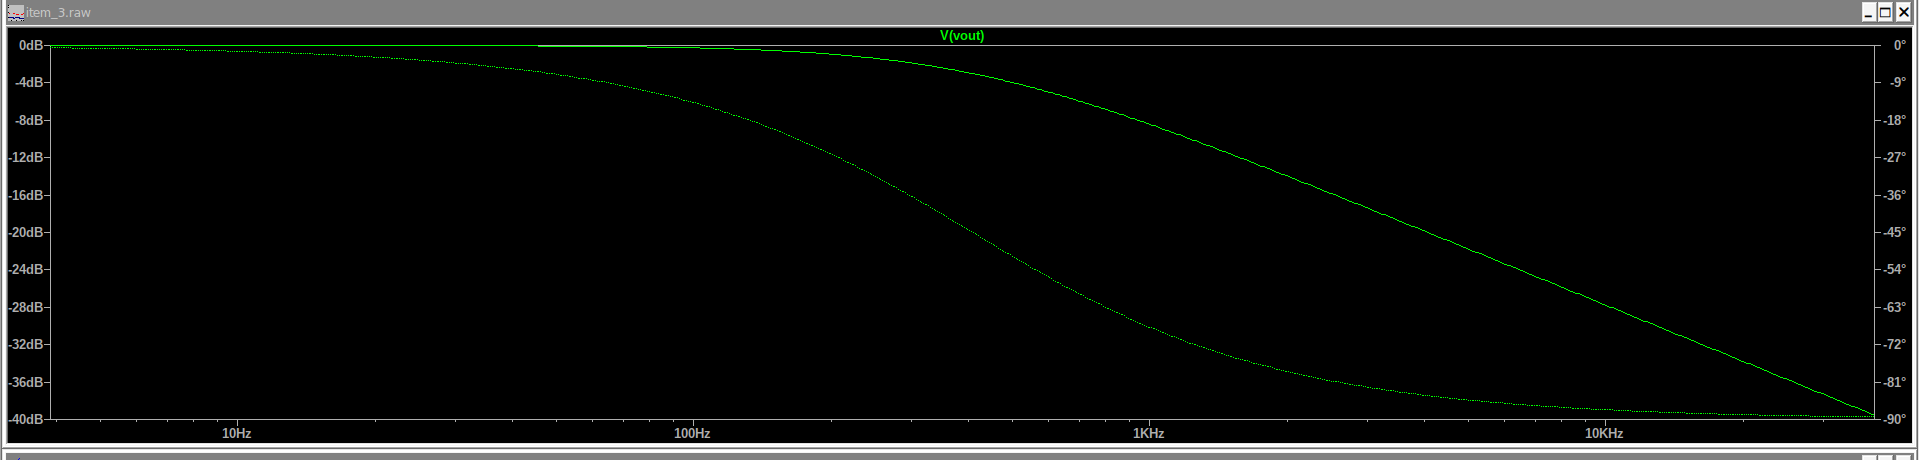
\includegraphics[width=\linewidth]{figuras/item_3_ltspice_corte.png}
\caption{Resposta em frequência do filtro RC no LTspice (\texttt{item\_3.asc}): magnitude em \si{\decibel} e fase de $V(v_{out})$.}
\label{fig:bode-rc}
\end{figure}

No RLC, os três valores de resistência produzem os resultados da Tabela~\ref{tab:rlc}. As respostas
ao degrau e em frequência aparecem nas Figuras~\ref{fig:rlc-tran} e \ref{fig:rlc-bode}.

\begin{center}
\captionof{table}{Resultados do RLC para os três passos de resistência.}
\label{tab:rlc}
\begin{tabular}{@{}rrrrl@{}}
\toprule
\textbf{$R$} & \textbf{$\zeta$} & \textbf{$f_d$} & \textbf{Pico do degrau} & \textbf{Regime} \\
\midrule
\SI{4,7}{\kilo\ohm} & 0,235 & \SI{15,470}{\kilo\hertz} & \SI{1,4679}{\volt} & subamortecido \\
\SI{12}{\kilo\ohm} & 0,600 & \SI{12,732}{\kilo\hertz} & \SI{1,0948}{\volt} & subamortecido \\
\SI{22}{\kilo\ohm} & 1,100 & --- & sem sobressinal & superamortecido \\
\bottomrule
\end{tabular}
\end{center}

\begin{figure}[htb]
\centering
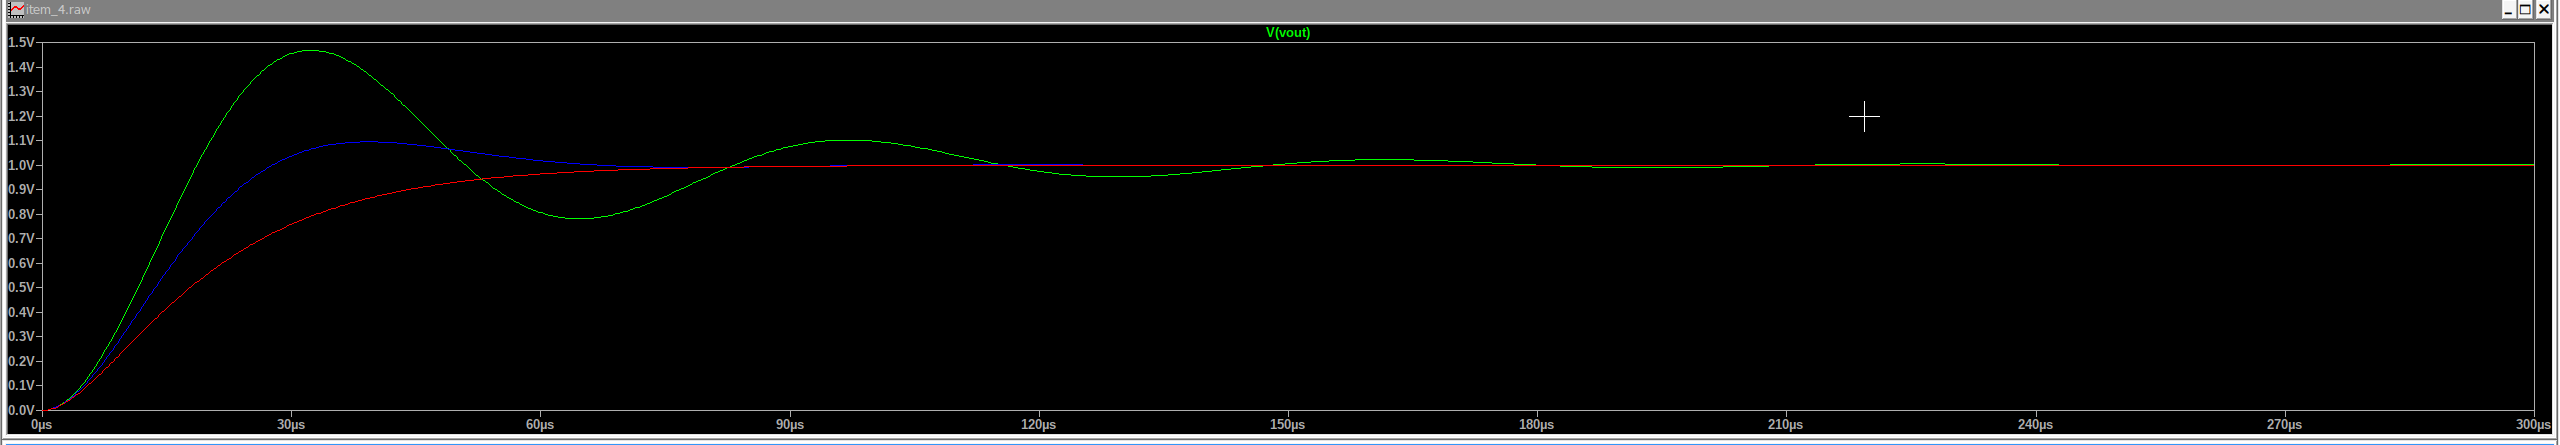
\includegraphics[width=\linewidth]{figuras/item_4_ltspice_vout_corte.png}
\caption{Resposta ao degrau do RLC no LTspice (\texttt{item\_4.asc}): $V(Vout)$ para $R=\SI{4,7}{\kilo\ohm}$, \SI{12}{\kilo\ohm} e \SI{22}{\kilo\ohm}.}
\label{fig:rlc-tran}
\end{figure}

\begin{figure}[htb]
\centering
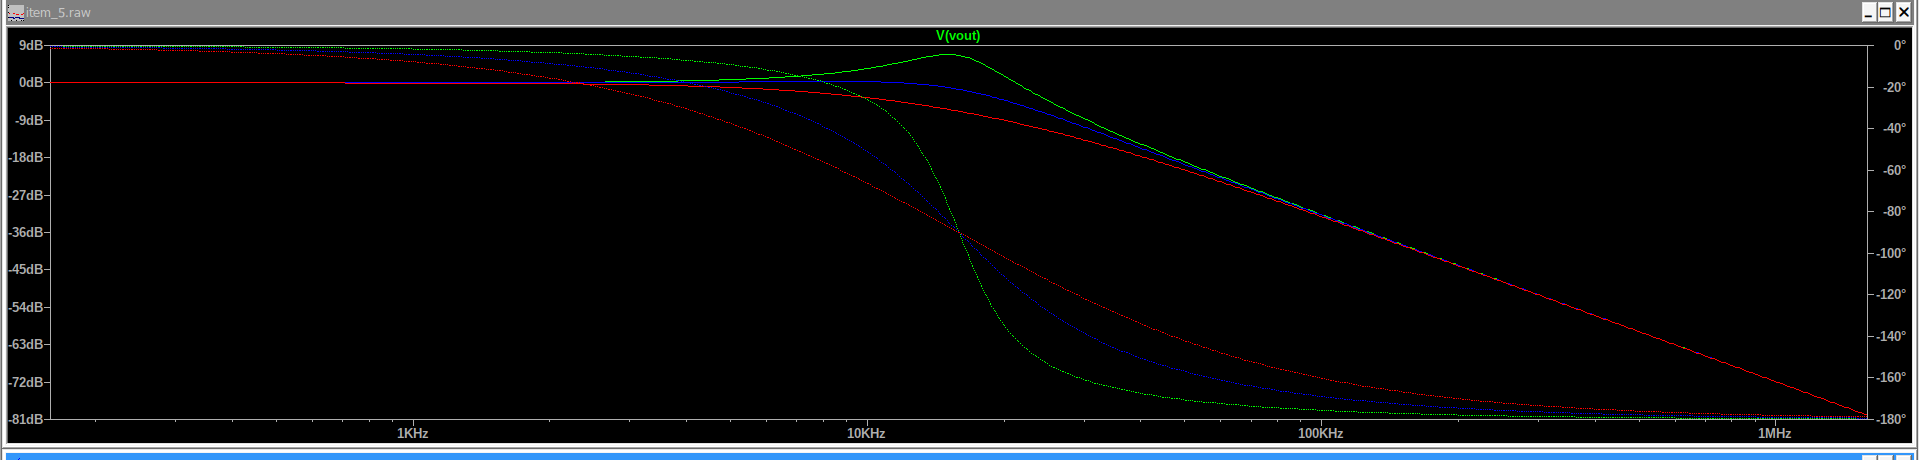
\includegraphics[width=\linewidth]{figuras/item_5_ltspice_corte.png}
\caption{Resposta em frequência do RLC no LTspice (\texttt{item\_5.asc}) para os três valores de resistência.}
\label{fig:rlc-bode}
\end{figure}

A onda quadrada e a saída filtrada são mostradas na Figura~\ref{fig:pulse}. A Tabela~\ref{tab:fft}
e a Figura~\ref{fig:fft} mostram que a atenuação aumenta com a ordem harmônica.

\begin{figure}[htb]
\centering
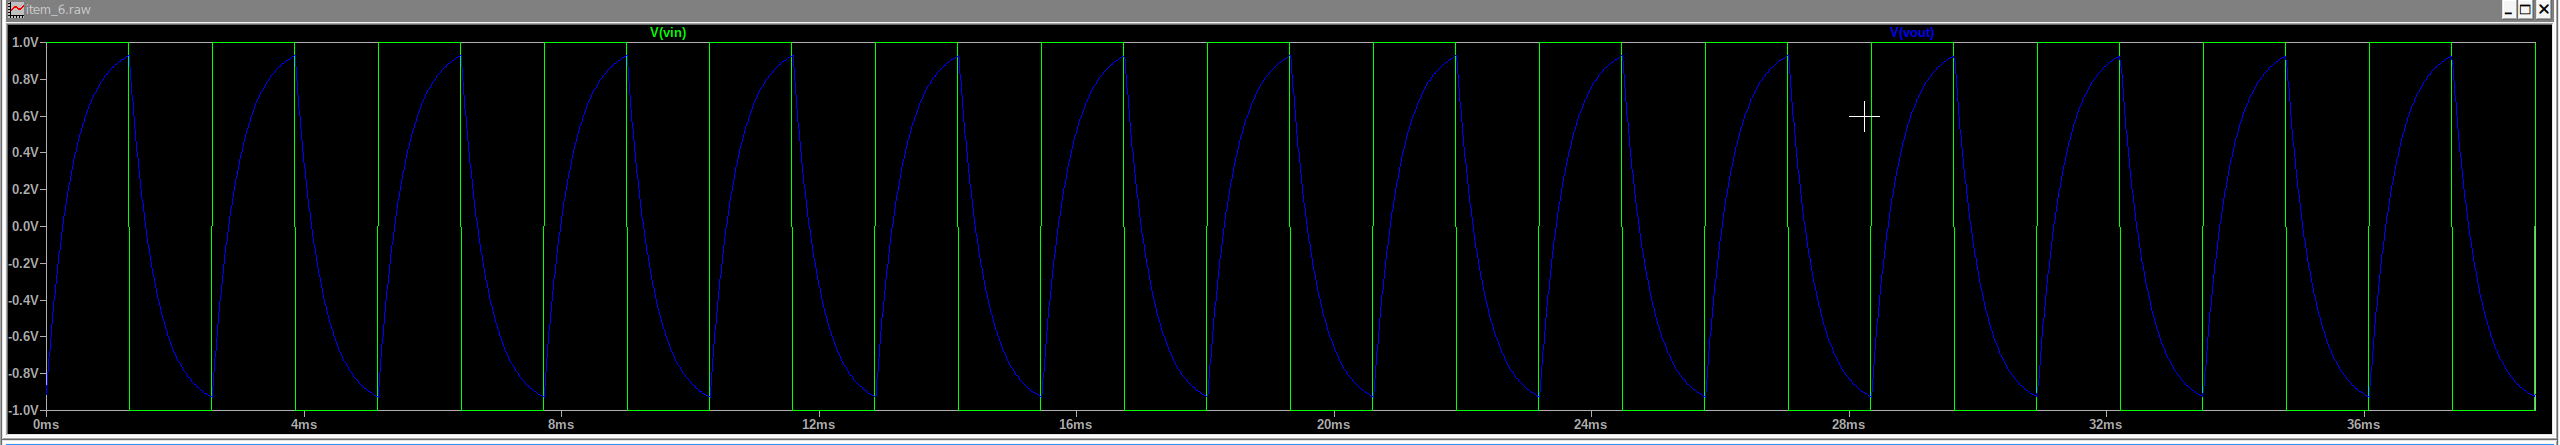
\includegraphics[width=\linewidth]{figuras/item_6_ltspice_tempo_real_corte.png}
\caption{Transiente do item 6 no LTspice (\texttt{item\_6.asc}): entrada quadrada $V(vin)$ e saída $V(vout)$ em regime permanente.}
\label{fig:pulse}
\end{figure}

\begin{center}
\captionof{table}{Cinco primeiras harmônicas ímpares.}
\label{tab:fft}
\begin{tabular}{@{}rrrr@{}}
\toprule
\textbf{$n$} & \textbf{Frequência} & \textbf{$V_{in,n}$} & \textbf{$V_{out,n}$} \\
\midrule
1 & \SI{388}{\hertz} & \SI{1,2732}{\volt} & \SI{0,9227}{\volt} \\
3 & \SI{1,164}{\kilo\hertz} & \SI{0,4244}{\volt} & \SI{0,1404}{\volt} \\
5 & \SI{1,940}{\kilo\hertz} & \SI{0,2546}{\volt} & \SI{0,0524}{\volt} \\
7 & \SI{2,716}{\kilo\hertz} & \SI{0,1819}{\volt} & \SI{0,0270}{\volt} \\
9 & \SI{3,492}{\kilo\hertz} & \SI{0,1415}{\volt} & \SI{0,0164}{\volt} \\
\bottomrule
\end{tabular}
\end{center}

\begin{figure}[htb]
\centering
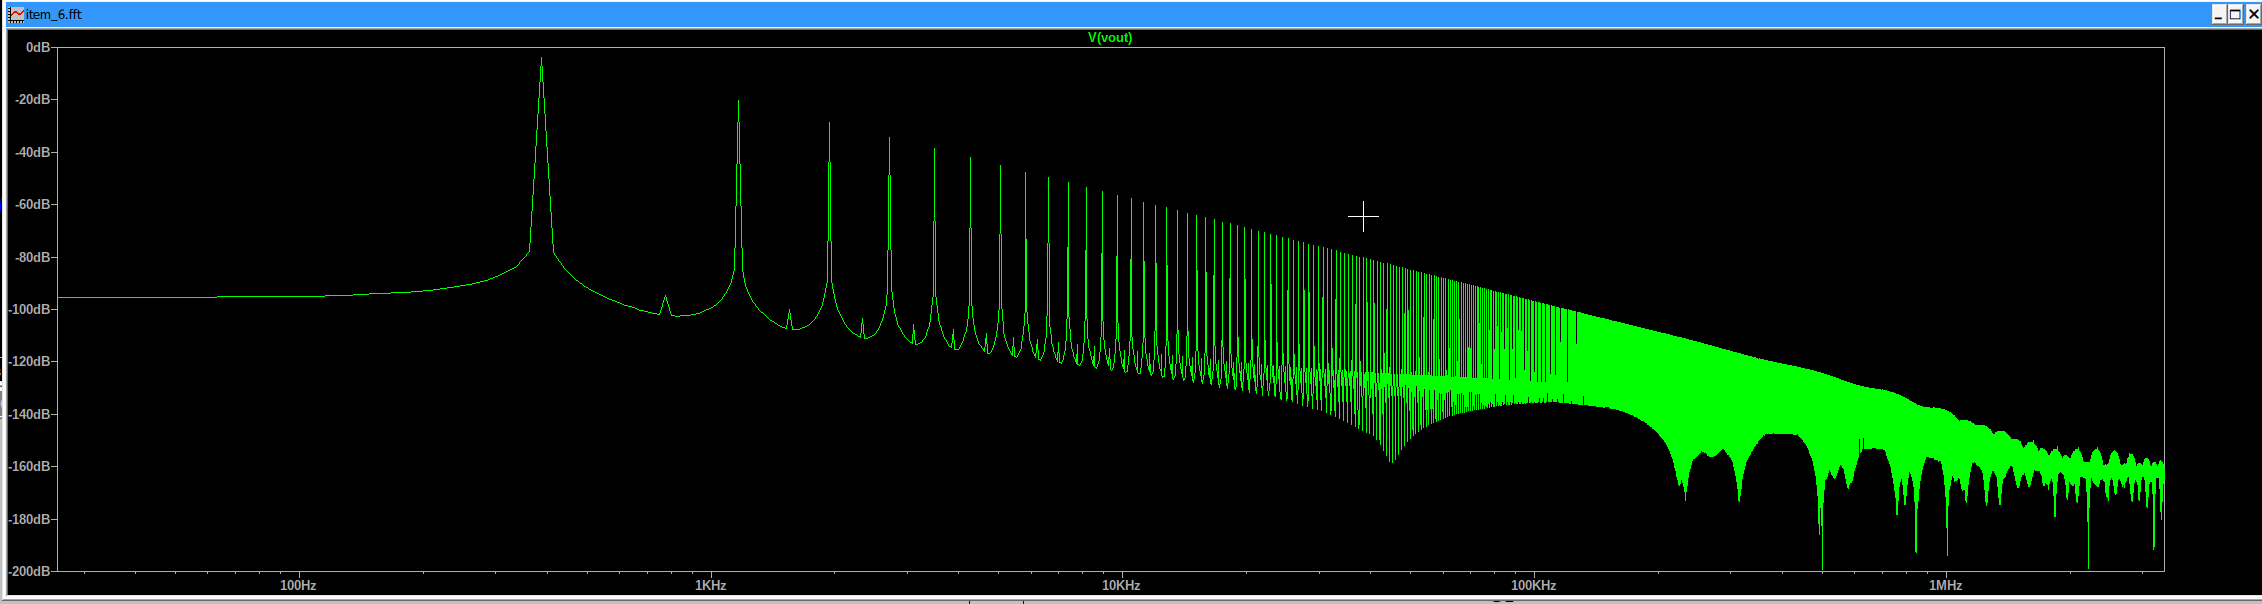
\includegraphics[width=\linewidth]{figuras/item_6_ltspice_fft_corte.png}
\caption{Transformada rápida de Fourier de $V(vout)$ no LTspice (\texttt{item\_6.asc}), com as harmônicas ímpares decrescendo e a atenuação imposta pelo filtro RC.}
\label{fig:fft}
\end{figure}

\FloatBarrier
\section{Discussão}

No divisor, $R_{th}=\SI{776,47}{\ohm}$ não é desprezível diante de $R_L=\SI{1}{\kilo\ohm}$.
Isso explica a queda de 43,71\% entre as condições sem carga e com carga. A saída carregada ainda
fica próxima da referência porque os valores de $R_1$ e $R_2$ foram escolhidos considerando esse
efeito, e não apenas a razão do divisor em vazio.

No RC, o corte efetivo difere da referência devido à passagem do resistor ideal de
\SI{4,101}{\kilo\ohm} para o valor E12 de \SI{3,9}{\kilo\ohm}. O desvio de 5,18\% é de projeto;
uma vez fixados os componentes, a curva segue exatamente o modelo de primeira ordem.

O RLC evidencia a ação da resistência sobre a energia armazenada. Com \SI{4,7}{\kilo\ohm}, o
sobressinal é 46,79\% e o Bode apresenta ressonância pronunciada. Em \SI{12}{\kilo\ohm}, o
sobressinal cai para 9,48\%. Com \SI{22}{\kilo\ohm}, acima de $R_{crit}$, desaparecem a oscilação
e o pico de ressonância.

Na onda quadrada, a fundamental é reduzida de \SI{1,273}{\volt} para \SI{0,923}{\volt}. A terceira
harmônica cai para \SI{0,140}{\volt}, e as seguintes são ainda menores. Essa remoção seletiva das
altas frequências produz as bordas arredondadas da saída. As harmônicas pares são nulas no modelo
ideal pela simetria da entrada.

Como o Roteiro 1 não possui bancada, a comparação é limitada ao cálculo analítico e ao modelo de
projeto. Não são avaliadas tolerâncias, perdas do indutor, resistência série do capacitor nem
carregamento dos instrumentos.

\section{Conclusão}

O objetivo de caracterizar as quatro topologias foi atingido. O divisor apresentou
\SI{3,642}{\volt} sob carga; o RC apresentou corte efetivo de \SI{408,1}{\hertz}; e a varredura do
RLC mostrou a transição de $\zeta=0,235$ para $\zeta=1,100$. A análise harmônica confirmou que o
filtro reduz progressivamente as componentes responsáveis pelas transições rápidas da onda
quadrada. Os resultados são coerentes com os modelos lineares ideais e com os valores registrados
nos arquivos do autor. A principal limitação é a ausência de medições reais, que impede avaliar
tolerâncias e efeitos parasitas.

\FloatBarrier
\section{Referências}

\begin{referencias}
\item ANALOG DEVICES. \emph{LTspice: simulador de circuitos eletrônicos}. Disponível em:
      \url{https://www.analog.com/en/resources/design-tools-and-calculators/ltspice-simulator.html}.
\item SEDRA, A.~S.; SMITH, K.~C. \emph{Microeletrônica}. 5.~ed. São Paulo: Pearson Prentice Hall, 2007.
\item BOYLESTAD, R.~L.; NASHELSKY, L. \emph{Dispositivos Eletrônicos e Teoria de Circuitos}.
      11.~ed. São Paulo: Pearson Education do Brasil, 2013.
\end{referencias}

\end{document}
